\documentclass[12pt]{article}
\usepackage{graphicx}

\usepackage{tikz}
\usetikzlibrary{}

\begin{document}

\section{Connecting nodes}

Try out the \textbackslash{}draw command to (roughly) replicate the connections
\vspace{1em}

\includegraphics{_img_src/00_connecting_nodes.pdf}

\vspace{1em}
\hrule 
\vspace{1em}

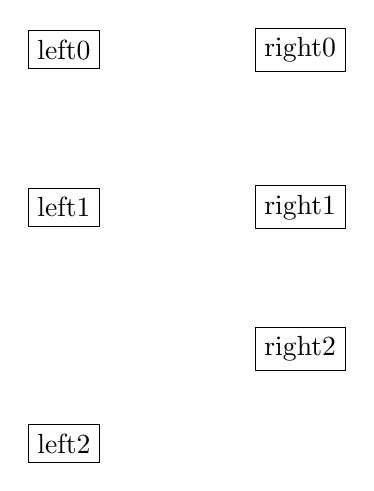
\begin{tikzpicture}
    \node[draw] (left0) at (0, 5) {left0};
    \node[draw] (right0) at (3, 5) {right0};
    \node[draw] (left1) at (0, 3) {left1};
    \node[draw] (right1) at (3, 3) {right1};
    \node[draw] (left2) at (0, 0) {left2};
    \node[draw] (right2) at (3, 1.2) {right2};

    %%%%%%%%%%%%%%%%%%%%%
    % Add your code here
    %%%%%%%%%%%%%%%%%%%%%
    
\end{tikzpicture}

\end{document}